%!TEX root = ../thesis.tex

\section{ルールベース制御器}
  ルールベース制御器は,2DLiDARの反射強度を入力とし,式\eqref{eq:angular_velocity}よりロボットのヨ―方向の角速度を出力する.これにより,ロボットは最大反射強度の方向に追従する.ルールベース制御器からの出力を\tabref{tab:output_from_rule-based_controller}と\figref{Fig:Action from rule-based controller}に示す.制御器では,角速度$\omega$が0 \,[rad/s]になると,カメラの中心に追従対象者が来る.

\vspace{-0.2cm}

  \begin{table}[!h]
    \centering
    \begin{tabular}{lcl}
        $\omega$ & : & ロボットのヨ―方向の角速度 [rad/s] \\
        $\theta_{\text{max}}$ & : & 2DLiDARの最大検出角度 [rad] \\
        $\theta$ & : & 2DLiDARの反射強度が最大の角度 [rad] \\
    \end{tabular}
  \end{table}

\vspace{-0.7cm}

  \begin{equation}
      \omega = \frac{1}{\theta_{\text{max}}} \times \theta
      \label{eq:angular_velocity}
  \end{equation}

\vspace{-0.5cm}

  \begin{table}[h]
    \caption{Output from rule-based controller}
    \label{tab:output_from_rule-based_controller}
    \centering
    \begin{tabular}{cccc}
    \hline
    Control rule {[}rad{]} & Linear velocity {[}m/s{]} & Angular velocity {[}rad/s{]} \\ 
    \hline
    \hline
    $\text{angle\_max} \geq \theta > 0$ & 0.2 & $1 \geq \omega > 0$ \\ 
    $0$ & 0.2 & $0$ \\ 
    $0 < \theta \leq \text{angle\_min}$ & 0.2 & $0 > \omega \geq -1$ \\ 
    \hline
    \end{tabular}
  \end{table}

  % \vspace{-0.5cm}

  \begin{figure}[h]
    \centering
    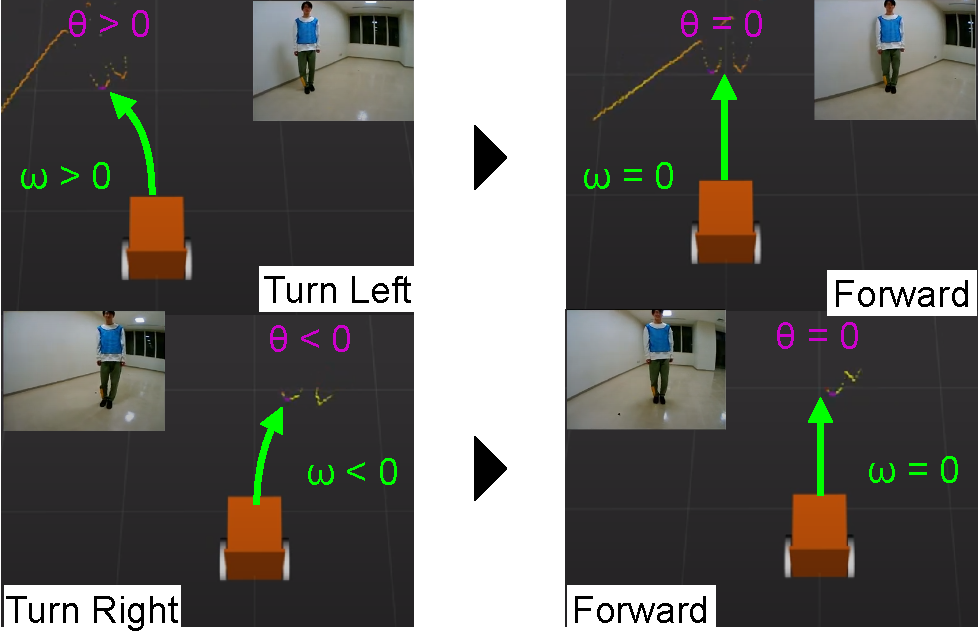
\includegraphics[height=6cm] {images/pdf/RobotGuidance_rule-based_controller}
    \captionsetup{justification=raggedright} % キャプションを左寄せに
    \caption{Action from rule-based controller}
    \label{Fig:Action from rule-based controller}
  \end{figure}

\newpage
